%!TeX spellcheck = en-GB

\documentclass[hyperref={colorlinks=true,urlcolor=blue,linkcolor=.},aspectratio=1610,mathserif]{beamer}
\usepackage[utf8]{inputenc}
\usepackage{pgfpages}
\usepackage{graphicx}
\usepackage{pdfpages}
\usepackage{tikz}
\usepackage[many]{tcolorbox}
\usepackage[autoplay,loop,keepaspectratio]{animate}
\usepackage{siunitx}
\sisetup{
	per-mode = power,
	round-mode = figures,
	round-precision = 3,
	scientific-notation = false,
	output-decimal-marker = {.},
	exponent-product = \times,
	separate-uncertainty = true,
	uncertainty-separator = ,
	output-product = \cdot,
	quotient-mode = fraction,
	range-phrase = -,
	range-units = single,
	inter-unit-product = \ensuremath{{\cdot{}}},
	number-unit-product = \,,
	multi-part-units = single,
	alsoload = synchem,
}
\DeclareSIUnit\atm{atm}
\usepackage{nth}
\usepackage{physics}
\usepackage{microtype}
\usepackage{chemfig}
\usepackage{tikzorbital}
\newcommand*\mathinhead[2]{\texorpdfstring{$\boldsymbol{#1}$}{#2}}
\newcommand{\me}{\mathrm{e}}
\usepackage{appendixnumberbeamer}
% Add total frame count to slides, optional. From Stefan,
% http://www.latex-community.org/forum/viewtopic.php?f=4&t=2173
\expandafter\def\expandafter\insertshorttitle\expandafter{%
	\insertshorttitle\hfill\insertframenumber\,/\,\inserttotalframenumber}
\usepackage{minted}
\setminted{fontsize=\scriptsize}
\usemintedstyle{tango}
\newcommand{\im}[3]{\inputminted[linenos=true, python3=true, firstline=#2, lastline=#3]{python}{#1}}
% ------------------------ Define note handout layout -------------------------
\newcommand{\pgflayout}{
	\pgfpagesphysicalpageoptions
	{%
		logical pages=2,%
		physical height=210mm,%
		physical width=297mm,%
	}%
	\pgfpageslogicalpageoptions{2}
	{%
		resized width=\pgfphysicalwidth,%
		resized height=\pgfphysicalheight,%
		center=\pgfpoint{.5\pgfphysicalwidth}{.25\pgfphysicalheight}%
	}%
	\pgfpageslogicalpageoptions{1}
	{%
		resized width=\pgfphysicalwidth,%
		resized height=\pgfphysicalheight,%
		center=\pgfpoint{.5\pgfphysicalwidth}{.70\pgfphysicalheight}%
	}%
}
% -----------------------------------------------------------------------------

% ---------------------------- Show note handout: -----------------------------
%\setbeameroption{show only notes}
%\pgflayout
% -----------------------------------------------------------------------------

% -------------------------- Define Beamer options ----------------------------
\beamertemplatenavigationsymbolsempty
\usefonttheme{serif}
\usecolortheme{beaver}

\setbeamertemplate{footline}
{%
	\begin{beamercolorbox}{section in foot}
		\begin{center}
			\vskip2pt\insertnavigation{\paperwidth}\vskip2pt
		\end{center}
	\end{beamercolorbox}%
}

\setbeamertemplate{note page}{%
	\vskip7em
	\begin{columns}[c]{\paperheight}
		\column{0.5\paperheight}
		\insertnote
		\column{0.5\paperheight}
		\insertslideintonotes{0.5}
	\end{columns}%
}

\setbeamersize{text margin left=10mm,text margin right=10mm}

\definecolor{DTUred}{cmyk}{0,0.91,0.72,0.23}
\definecolor{itemcolor}{cmyk}{0,0,0,0.56}
\definecolor{blockbodycolor}{cmyk}{0,1,1,0.5}
\definecolor{White}{cmyk}{0,0,0,0}
\setbeamercolor{titlelike}{fg=DTUred}
\setbeamercolor{section in head/foot}{fg=DTUred}
\setbeamercolor{section in toc}{fg=DTUred}
\setbeamercolor{itemize item}{fg=itemcolor}
\setbeamercolor{redbox}{fg=White,bg=blockbodycolor}
\setbeamercolor{description item}{fg=DTUred}

% -----------------------------------------------------------------------------

\title{Quantum Transport in Nanoporous Graphene}
\subtitle{Bachelor defense}
\author{\scshape\centering Christoffer Vendelbo Sørensen (s163965) \vskip\vspace{7.5mm} 
\includegraphics[width=1cm]{Figures/DTU3CMYK.eps}}
\date{\scshape June 25, 2019}

%\AtBeginSection[]
%{
%  \begin{frame}<beamer>
%    \frametitle{Outline for section \thesection}
%    \tableofcontents[currentsection]
%  \end{frame}
%}

\begin{document}

\begin{frame}[plain]
	\titlepage
\end{frame}

\begin{frame}
	\frametitle{Outline}
	\tableofcontents
\end{frame}

\section{Introduction}
\subsection{Project aim and nanoporous graphene}
\begin{frame}{Project aim}
    \centering
	    \begin{beamercolorbox}[sep=1em,wd=15cm]{redbox}
		``Development of tight-binding routines in Python in order to understand electron transport in novel nanoporous graphene devices (NPGs)''
	    \end{beamercolorbox}
\end{frame}

\begin{frame}{Nanoporous graphene}
	\centering
	\begin{columns}[c]
		\column{.7\textwidth}
		\begin{itemize}
			\item Planar graphene sheets
			\item Periodically removed atoms
			\item Ribbons and bridges
			      %\item Bridge chemistry \(\rightarrow\) current control
			\item Ballistic electron movement
			\item Potential for controlling currents on nanoscale
		\end{itemize}
		\column{.7\textwidth}
		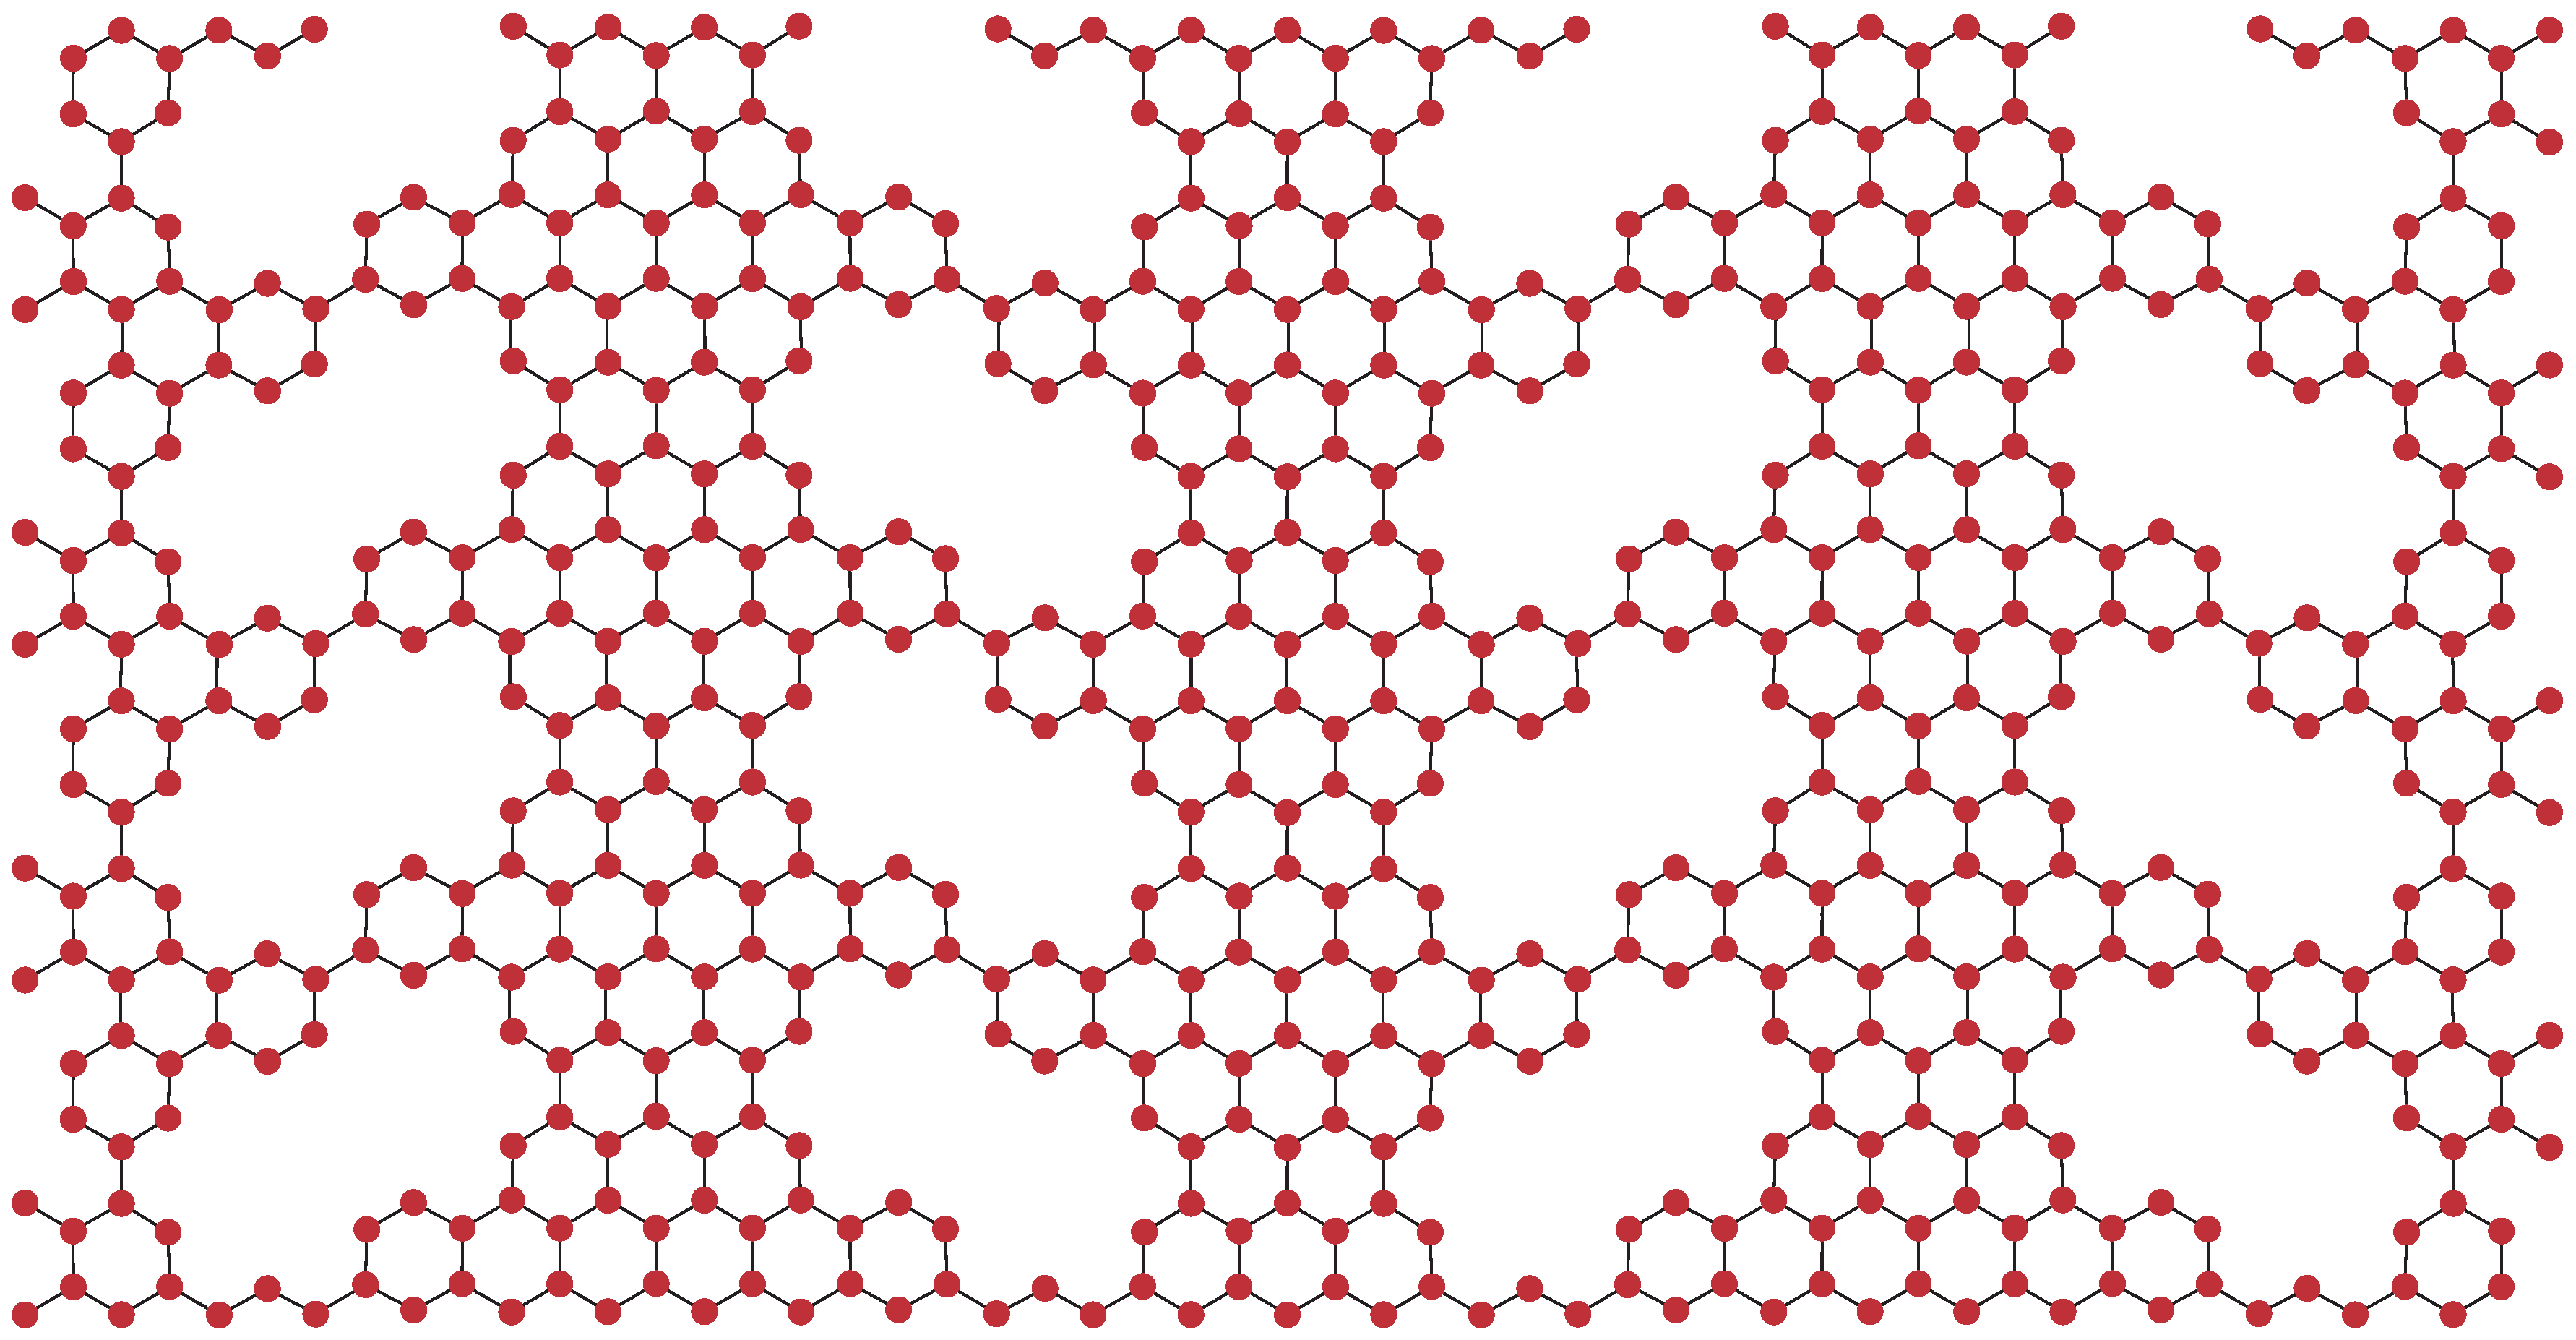
\includegraphics[width=.6\textwidth]{Figures/NPGintroGraphic.eps}
	\end{columns}
\end{frame}

\section{Tight Binding}
\subsection{\mathinhead{\pi}{\pi}-orbitals, \mathinhead{\pi}{\pi}-electrons and the TB approximation}
\begin{frame}{\mathinhead{\pi}{\pi}-orbitals and \mathinhead{\pi}{\pi}-electrons}
	\centering
	\begin{columns}[c]
		\column{.7\textwidth}
		\begin{itemize}
			\item In plane electrons are bound
			\item 1 \(p_z\)-electron per site
			\item ``Tightly bound'' hops between sites
		\end{itemize}
		\column{.7\textwidth}
		\resizebox{.4\textwidth}{!}{
			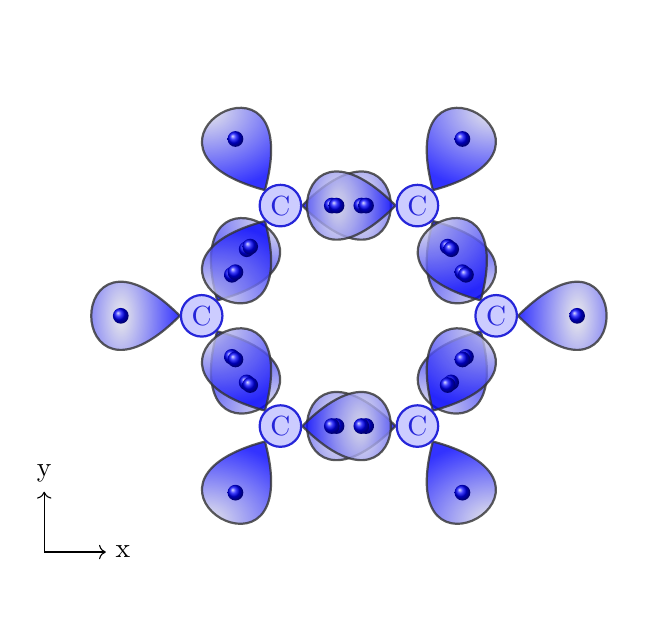
\begin{tikzpicture}
				\node (x) at (-1,-3) {x};
				\node (y) at (-2,-2) {y};
				\draw[->] (-2,-3) -- (x);
				\draw[->] (-2,-3) -- (y);
				\satom[name=C, color=blue, pos={(0,0)}]{
					blue/60/north east/2/1,
					blue/180/west/1,
					blue/300/south east/2/1
				}
				\satom[name=C, color=blue, pos={(1,1.4)}]{
					blue/0/east/2/1,
					blue/120/north west/1,
					blue/240/south west/2/1
				}
				\satom[name=C, color=blue, pos={(2.74,1.4)}]{
					blue/60/north east/1,
					blue/180/west/2/1,
					blue/300/south east/2/1
				}
				\satom[name=C, color=blue, pos={(3.74,0)}]{
					blue/0/east/1,
					blue/120/north west/2/1,
					blue/240/south west/2/1
				}
				\satom[name=C, color=blue, pos={(2.74,-1.4)}]{
					blue/60/north east/2/1,
					blue/180/west/2/1,
					blue/300/south east/1
				}
				\satom[name=C, color=blue, pos={(1,-1.4)}]{
					blue/0/east/2/1,
					blue/120/north west/2/1,
					blue/240/south west/1
				}
			\end{tikzpicture}}
		\pgfdeclarelayer{background}
		\pgfdeclarelayer{middle}
		\pgfdeclarelayer{foreground}
		\pgfsetlayers{background,middle,main,foreground}
		\vskip
		\resizebox{.4\textwidth}{!}{
			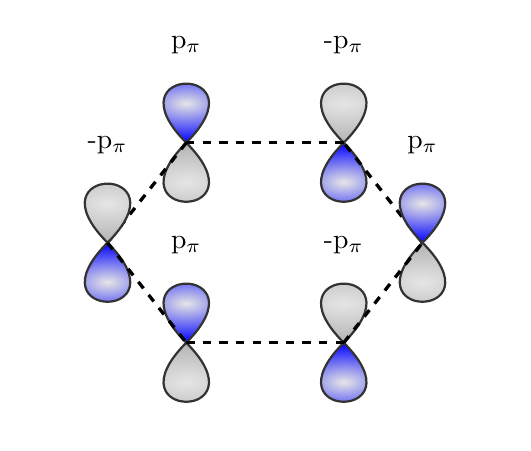
\begin{tikzpicture}
				\begin{pgfonlayer}{background}
					\orbital[pos = {(6,6)}]{-pz}
					\node[above] at (6,7) {-p$_\pi$};
					\orbital[pos = {(4,6)}]{pz}
					\node[above] at (4,7) {p$_\pi$};
					\draw[dashed, very thick] (6,6) -- (4,6);
					\draw[dashed, very thick] (7,4.73) -- (6,6);
					\draw[dashed, very thick] (4,6) -- (3,4.73);
				\end{pgfonlayer}
				\orbital[pos = {(7,4.73)}]{pz}
				\node[above] at (7,5.73) {p$_\pi$};
				\orbital[pos = {(3,4.73)}]{-pz}
				\node[above] at (3,5.73) {-p$_\pi$};
				\begin{pgfonlayer}{foreground}
					\orbital[pos = {(4,3.46)}]{pz}
					\node[above] at (4,4.46) {p$_\pi$};
					\orbital[pos = {(6,3.46)}]{-pz}
					\node[above] at (6,4.46) {-p$_\pi$};
					\draw[dashed, very thick] (4,3.46) -- (6,3.46);
				\end{pgfonlayer}
				\draw[dashed, very thick] (6,3.46) -- (7,4.73);
				\draw[dashed, very thick] (3,4.73) -- (4,3.46);
			\end{tikzpicture}}
	\end{columns}
\end{frame}

\begin{frame}{TB approximation}
	\centering
	\begin{columns}[c]
		\column{.5\textwidth}
		\begin{itemize}
			\item Electrons tightly bound to sites
			\item Hops with potential
			\item Average electron energy on site
			\item The Hamiltonian is a hop matrix
		\end{itemize}
		\column{.7\textwidth}
		\begin{align}
			V_{pp\pi}  & = \bra{\phi_{\pi}(m)}\vu{H}\ket{\phi_{\pi}(n)}\nonumber \\
			\epsilon_0 & = \bra{\phi_{\pi}(i)}\vu{H}\ket{\phi_{\pi}(i)}\nonumber
		\end{align}
	\end{columns}
	\note{\(\epsilon_0 = 0\)}
	\note{\(\Psi_{\mathrm{MO}} &= \sum_{\alpha,R}c_{\alpha,R}\phi_{\alpha}(R)\)}
\end{frame}

\begin{frame}{Hamiltonian for benzene}
	\centering
	\begin{columns}[c]
		\column{.7\textwidth}
		\begin{align}
			\mqty{                            \\ \\ \\ \vb{H} = V_{pp\pi}\\ \\ \\} \ \mqty{						&  \mqty{1 & 2 & 3 & 4 & 5 & 6} \\
				\mqty{1                           \\ 2 \\ 3 \\ 4 \\ 5 \\ 6} &	\mqty*(0 & 1 & 0 & 0 & 0 & 1 \\
			1 & 0 & 1 & 0 & 0 & 0             \\
			0 & 1 & 0 & 1 & 0 & 0             \\
			0 & 0 & 1 & 0 & 1 & 0             \\
			0 & 0 & 0 & 1 & 0 & 1             \\
			1 & 0 & 0 & 0 & 1 & 0)} \nonumber
		\end{align}
		\column{.5\textwidth}
		\begin{tikzpicture}
			\chemfig{1*6(-2-3-4-5-6-)}
		\end{tikzpicture}
	\end{columns}
\end{frame}

\section{The Hamiltonian}
\subsection{Onsites, hops and the full TB Hamiltonian}
\begin{frame}{Creating the first Hamiltonian}
	\begin{center}
		\begin{columns}[c]
			\column{.5\textwidth}
			\begin{itemize}
				\item Atom coordinates
				\item Interatomic distances
				\item Applying potential
			\end{itemize}
			\note{Outer product: Nested lööps}
			\column{.9\textwidth}
			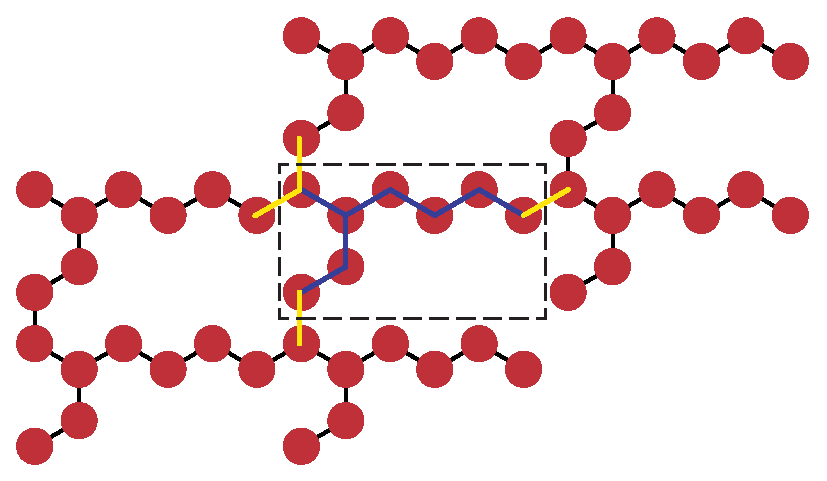
\includegraphics[width=.7\textwidth]{Figures/atomreffig.eps}
		\end{columns}
	\end{center}
	\begin{columns}[t]\column{.05\textwidth}\column{.9\textwidth}\im{Listings/Functions.py}{33}{38}\end{columns}
\end{frame}

\begin{frame}{Hopping matrices}
	\centering
	\begin{columns}[c]
		\column{.7\textwidth}
		\begin{itemize}
			\item Shift by lattice vector
			\item Resulting matrices: \(\vb{h_0}, \vb{V}, \vb{V}^{\dagger}\)
		\end{itemize}
		\column{.7\textwidth}
		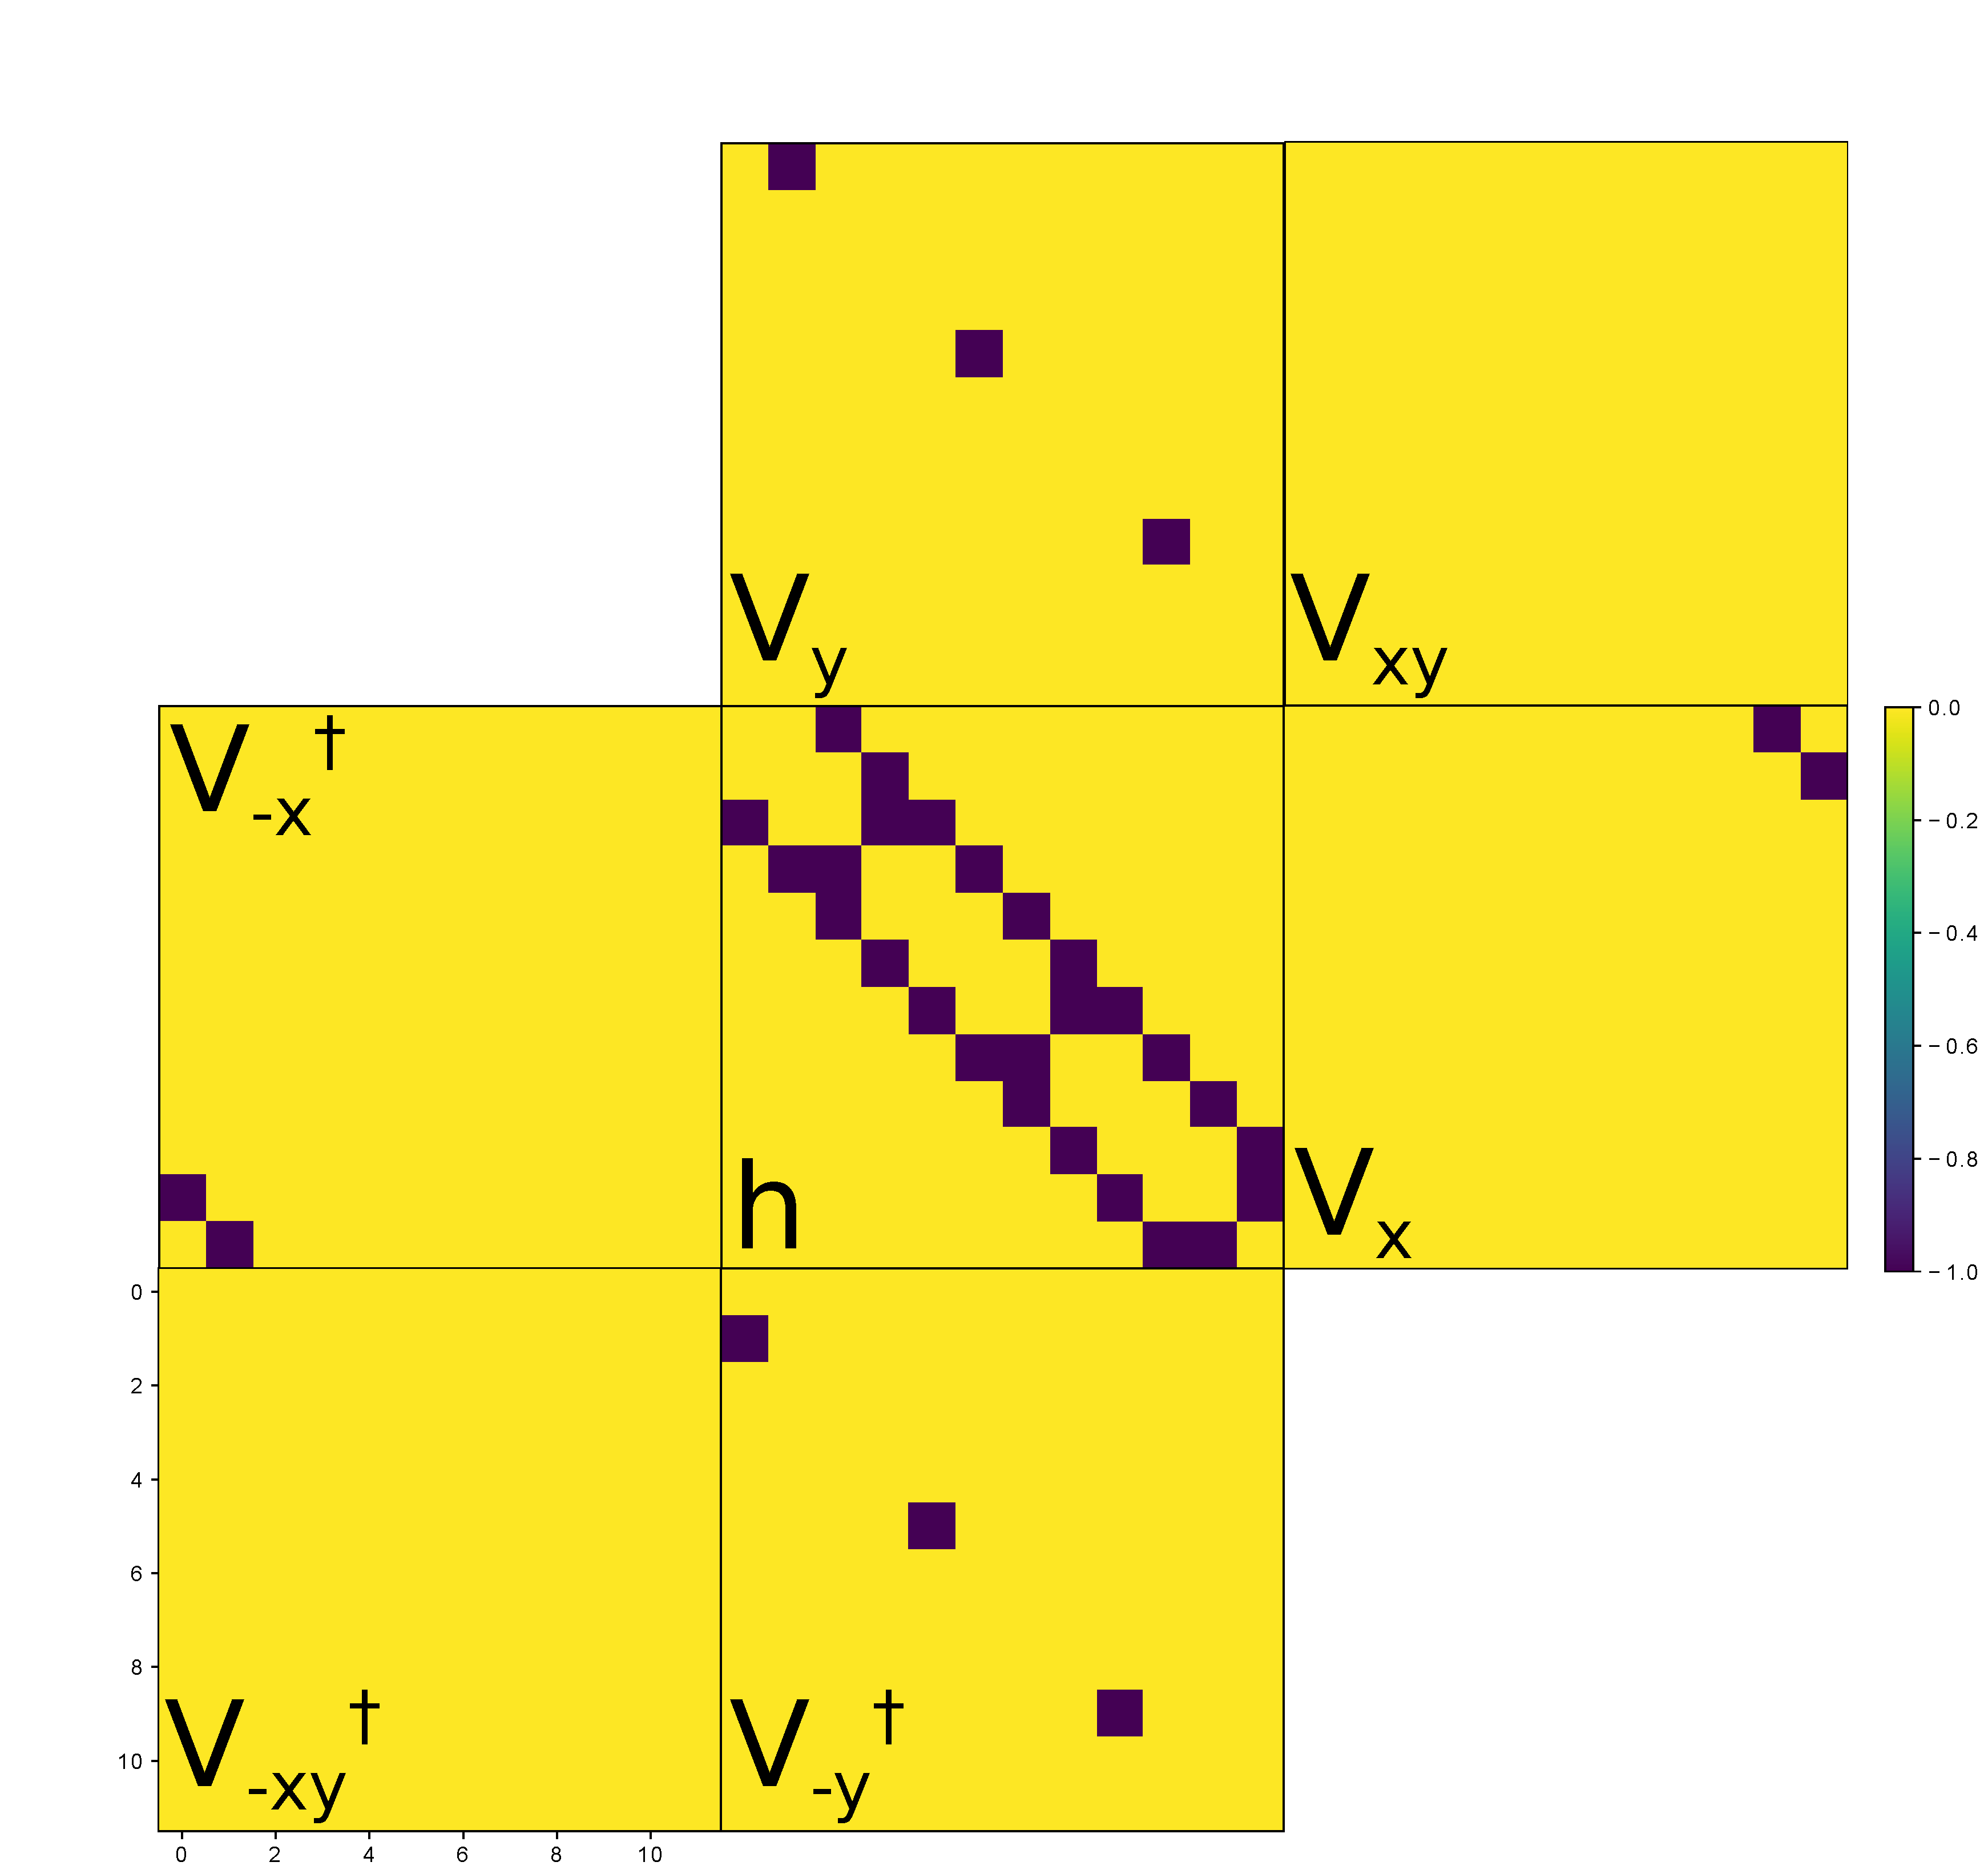
\includegraphics[width=\textwidth]{Figures/stitch.eps}
	\end{columns}
\end{frame}

\begin{frame}{Full Hamiltonian and first band plots}
	\begin{overprint}
		\onslide<1>
		\begin{align}
			\vb{H}(k_x,k_y) \vb*{\phi}_k & = \vb*{\epsilon}_n\pqty{k_x,k_y}\vb*{\phi}_k\nonumber                                                               \\
			\vb{H}(k_x,k_y) = \vb{h}_0   & + (\vb{V}_{x}e^{-ik_x} + \vb{V}_{x}^{\dagger}e^{ik_x} + \vb{V}_{y}e^{-ik_y} + \vb{V}_{y}^{\dagger}e^{ik_y}\nonumber \\
			                             & + \vb{V}_{xy}e^{-ik_x}e^{-ik_y} + \vb{V}_{xy}^{\dagger}e^{ik_x}e^{ik_y})\nonumber
		\end{align}
		\im{Listings/Functions.py}{73}{80}
		\onslide<2>
		\begin{columns}[c]
			\column{.7\textwidth}
			\begin{align}
				\qq{X:} \vb{H}_{X} = \vb{h}_0 + ( & \vb{V}_{x}e^{ik_x} + \vb{V}_{x}^{\dagger}e^{-ik_x} + \vb{V}_{y} + \vb{V}_{y}^{\dagger}\nonumber \\
				+\                                & \vb{V}_{xy}e^{ik_x} + \vb{V}_{xy}^{\dagger}e^{-ik_x}) \nonumber                                 \\
				\qq{Y:} \vb{H}_{Y} = \vb{h}_0 + ( & \vb{V}_{x} + \vb{V}_{x}^{\dagger} + \vb{V}_{y}e^{-ik_y} + \vb{V}_{y}^{\dagger}e^{ik_y}\nonumber \\
				+\                                & \vb{V}_{xy}e^{-ik_y} + \vb{V}_{xy}^{\dagger}e^{ik_y}) \nonumber
			\end{align}
			\column{.7\textwidth}
			\includegraphics[width=.65\textwidth]{Figures/BetaBandstructures.eps}
		\end{columns}
	\end{overprint}
\end{frame}

\section{Green's functions and recursion}
\subsection{Green's matrix, recursion and LDOS}

\begin{frame}{Green's matrix}
	\begin{center}
		\begin{columns}[c]
			\column{.7\textwidth}
			\begin{itemize}
				\item Solution to the Sc\"{o}dinger Equation
				\item Propagator
			\end{itemize}
			\column{.7\textwidth}
			\begin{align*}
				 & [(E+i\eta)\vb{1}-\vb{H}]\vb{G}(E)=\vb{1}        \\
				 & \downarrow                                      \\
				 & \vb{G}(E)=\vb{1}([(E+i\eta)\vb{1}-\vb{H}])^{-1}
			\end{align*}
		\end{columns}
	\end{center}
\end{frame}

\begin{frame}{Recursion}
	\begin{overprint}
		\onslide<1>
		\begin{center}
			\begin{columns}[c]
				\column{.7\textwidth}
				\begin{itemize}
					\item Semi-infinite chain
				\end{itemize}
				\begin{align*}
					 & \begin{pmatrix}
						z\mathbf{1}-\mathbf{H}_c & -\mathbf{V}^{\dagger} \\ -\mathbf{V} & (z-\varepsilon')\mathbf{1}
					\end{pmatrix}
					\begin{pmatrix}
						\mathbf{X}      & \mathbf{G}_{0c} \\
						\mathbf{G}_{c0} & \mathbf{G}_{00}
					\end{pmatrix}
					=
					\begin{pmatrix}
						\mathbf{1} & \mathbf{0} \\
						\mathbf{0} & \mathbf{1}
					\end{pmatrix}
				\end{align*}
				\begin{align*}
					\mathbf{G}_{00}(z) & = \left[(z-\varepsilon')-\vb{V}(z\vb{1}-\vb{H}_c)\vb{V}^{\dagger}\right]^{-1} \\
					                   & = (z-\varepsilon'-\Sigma(z))^{-1}                                             \\
					                   & \qq{where}                                                                    \\
					z                  & = E+i\eta                                                                     \\
				\end{align*}
				\column{.7\textwidth}
				\begin{align*}
					a_0           & = \vb{V}^{\dagger}, \quad b_0 = \vb{V}                        \\
					e_{s0}        & = \vb{h}_s, \quad e_0\ = \vb{h}                               \\
					              & \qq{in loop:}                                                 \\
					a_1           & = a_0 \times g_0 \times a_0                                   \\
					b_1           & = b_0 \times g_0 \times b_0                                   \\
					e_1           & = e_0 + a_0 \times g_0 \times b_0 + b_0 \times g_0 \times a_0 \\
					e_{1s}        & = e_{0s} + a_0 \times g_0 \times b_0                          \\
					g_1           & = \pqty{z-e_1}^{-1}                                           \\
					\vb{\Sigma}_R & = e_s - h                                                     \\
					\vb{\Sigma}_L & = e - h - \vb{\Sigma}_R                                       \\
					\vb{G00}      & = \pqty{z-e_s}^{-1}
				\end{align*}
			\end{columns}
		\end{center}
		\onslide<2>
		\im{Listings/Functions.py}{92}{109}
	\end{overprint}
\end{frame}

\begin{frame}{LDOS}
	\centering
	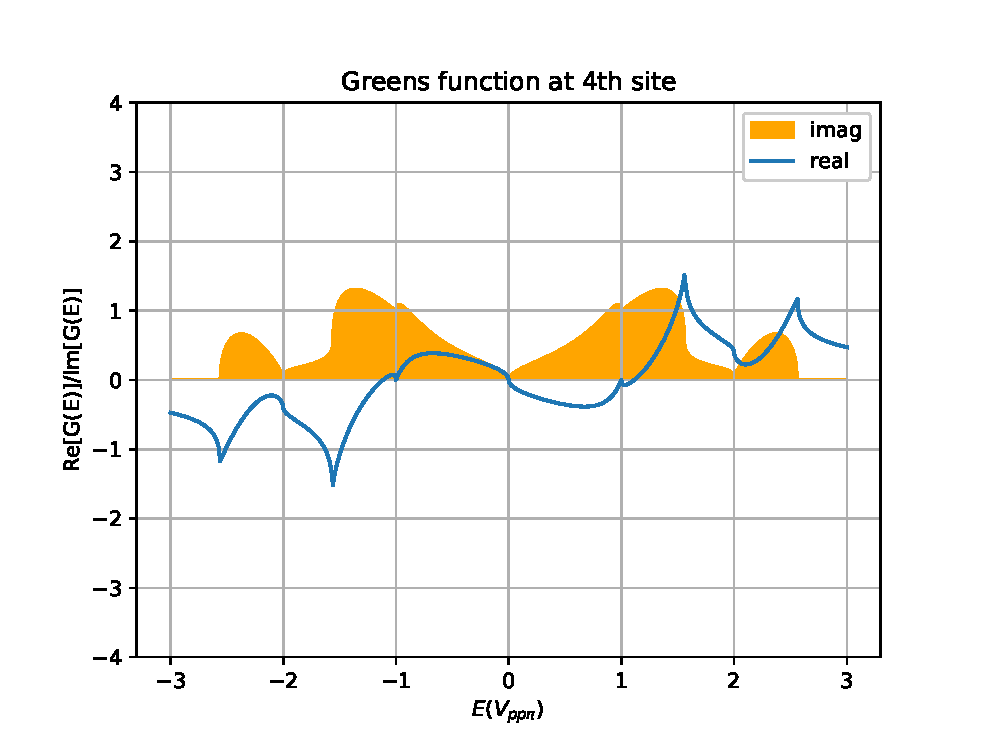
\includegraphics[width=.7\textwidth]{Figures/BetaimrealTE.eps}
	\im{Listings/SelfEnergyByRecursion.py}{64}{68}
\end{frame}

\section{Transmission}
\subsection{Device Green's functions, left/right geometry, rate matrices and spectral functions.}

\begin{frame}{Translating from system to matrices}
\centering
\begin{overprint}
\onslide<1>
		    Transmission is the probability of an electron being transported through a specific region for a specific range of energies.
\onslide<2>
			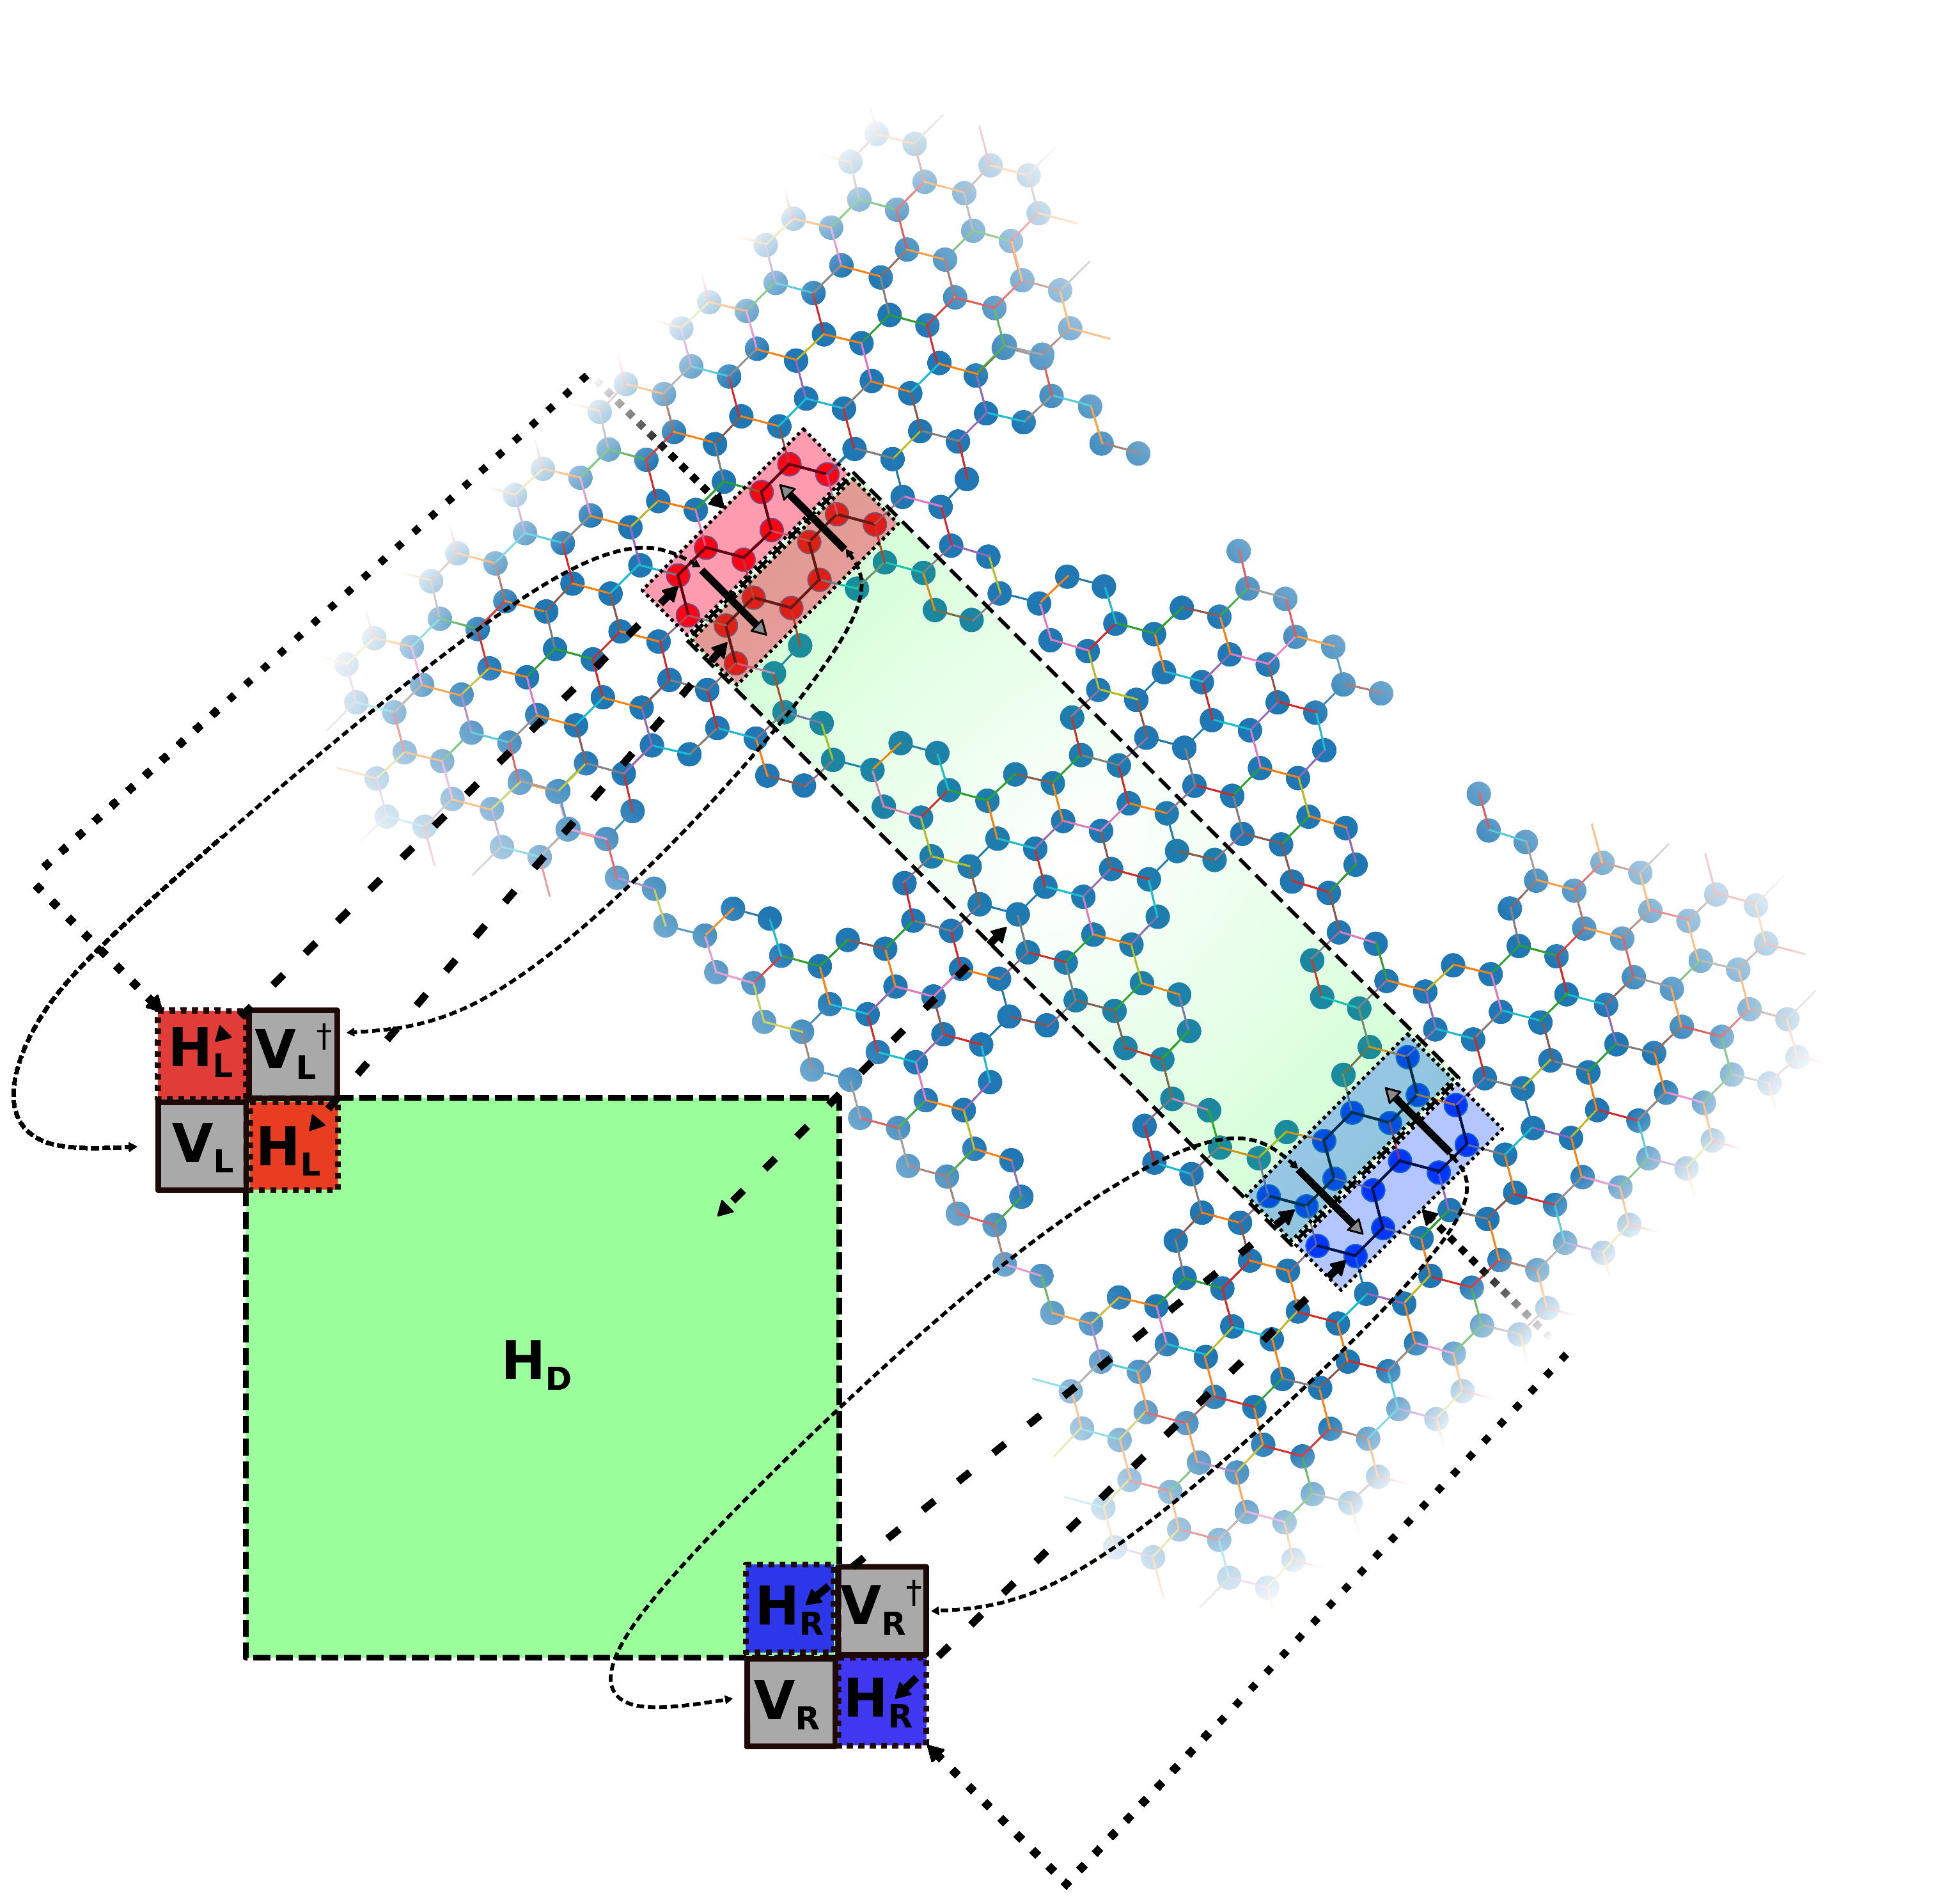
\includegraphics[width=\textwidth]{Figures/illu.eps}
\end{overprint}
\end{frame}

\begin{frame}{The left and right self-energy}
    \centering
   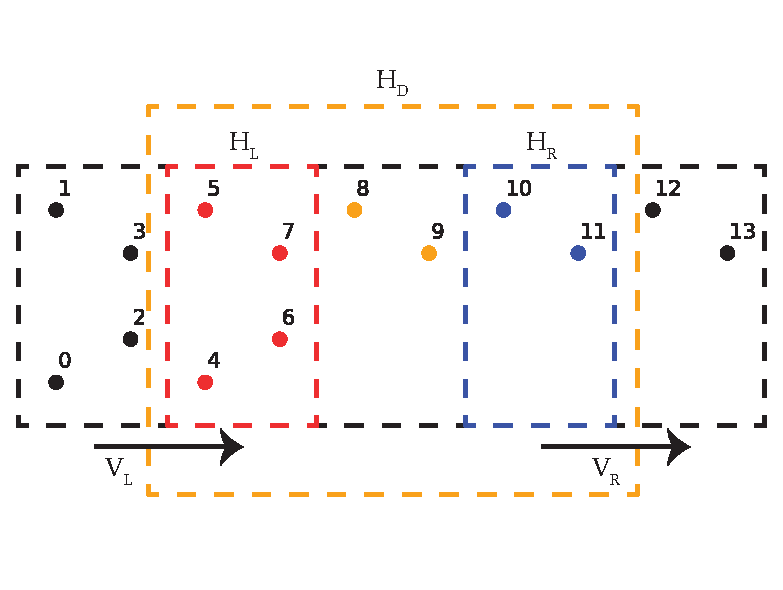
\includegraphics[width=.9\textwidth]{Figures/2DHam.eps}
    \im{Listings/Functions.py}{210}{212}
\end{frame}

\begin{frame}{Getting Transmission}
    \centering
\begin{overprint}
\onslide<1>
\begin{align*}
    \vb{G}_D &= \bqty{\vb{1}\pqty{E+i\eta}-\vb{H}_D - \vb{\Sigma}_L(E)-\vb{\Sigma}_R(E)}^{-1}\\
    \vb{\Gamma}_{L,R} &= i\pqty{\vb{Sigma}_{L,R} - \vb{\Sigma}_{L,R}^{\dagger}}
\end{align*}
\im{Listings/Functions.py}{225}{228}
\onslide<2>
\begin{align*}
    T(E) = \mathrm{Tr}\bqty{\vb{\Gamma}_R\vb{G}_D\vb{\Gamma}_L\vb{G}^{\dagger}}(E)
\end{align*}
    \im{Listings/Functions.py}{240}{243}
\onslide<3>
    \begin{columns}[c]
    \column{.7\textwidth}
    \begin{itemize}
        \item Text1
        \item Text2
        \item Text3
    \end{itemize}
    \column{.7\textwidth}
    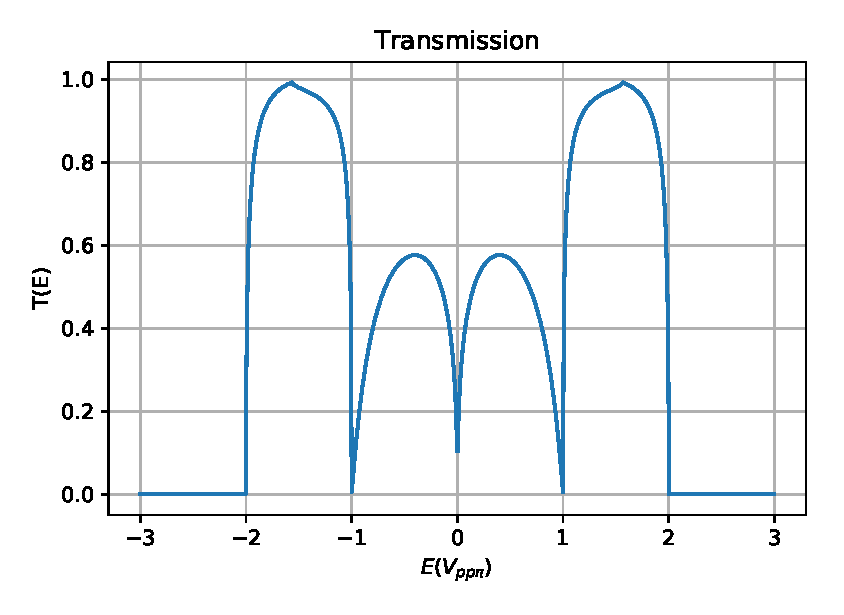
\includegraphics[width=\textwidth]{Figures/BetaTE.eps}
    \end{columns}
\end{overprint}
\end{frame}

\subsection{Transmission in 2D}

\begin{frame}{Transmission in 2D}
\centering
\begin{columns}[c]
\column{.7\textwidth}
		    \begin{align*}
		        \vb{H} = \vb{h} + \vb{V}\me^{ik_{\perp}} + \vb{V}^{\dagger} \me^{i\pqty{-k_{\perp}}}
		    \end{align*}
		    \im{Listings/Functions.py}{250}{253}
\column{.7\textwidth}
			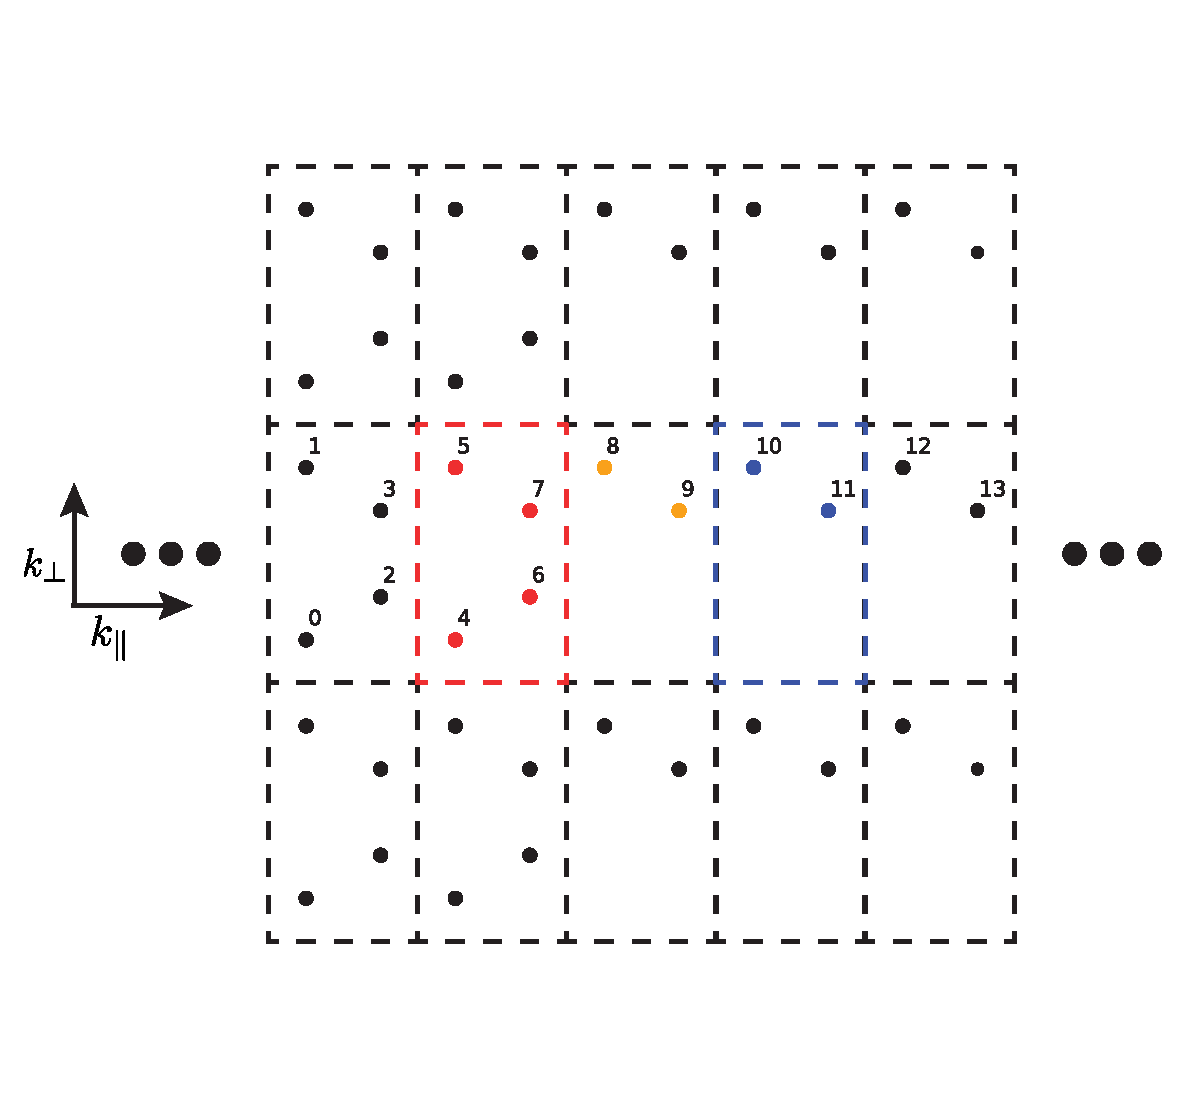
\includegraphics[width=\textwidth]{Figures/2DTrans.eps}
\end{columns}
\end{frame}

\begin{frame}{Code validity}
\centering
\begin{overprint}
\onslide<1>
\centering
\begin{align*}
		k = \frac{\pi}{2}
\end{align*}
\begin{columns}[t]
    \column{.7\textwidth}
    \includegraphics[width=\textwidth]{Figures/NPGNormal_pi-half.eps}
    \column{.7\textwidth}
    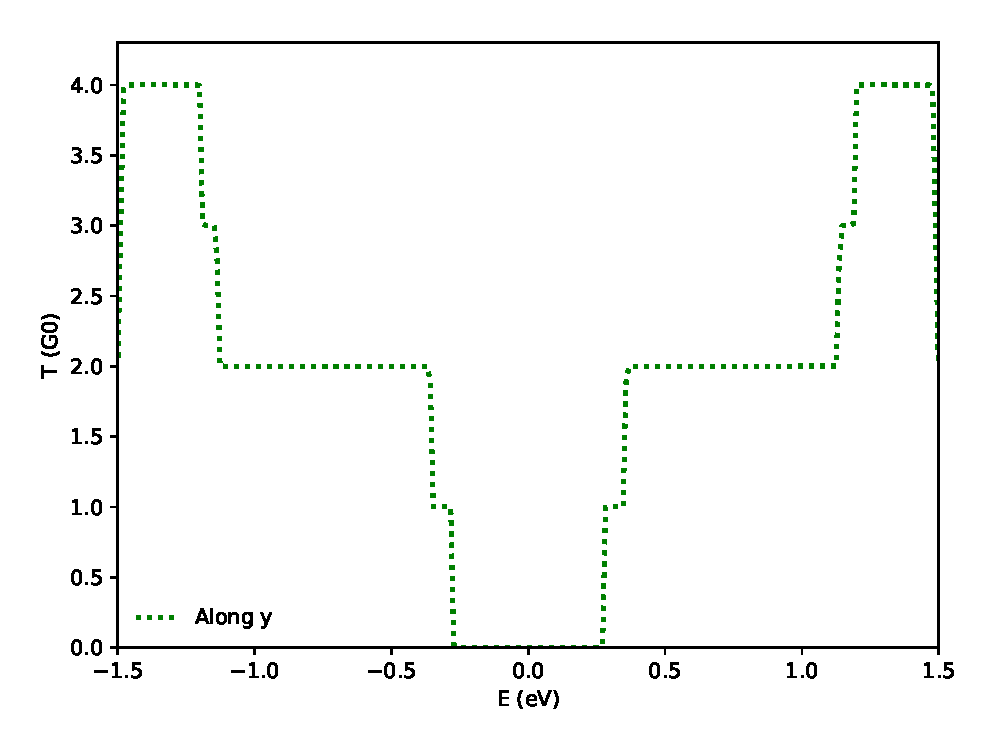
\includegraphics[width=.97\textwidth]{Figures/txy_pi-half.eps}
\end{columns}
\onslide<2>
\centering
\begin{align*}
		k = \pi
\end{align*}
\begin{columns}[t]
    \column{.7\textwidth}
    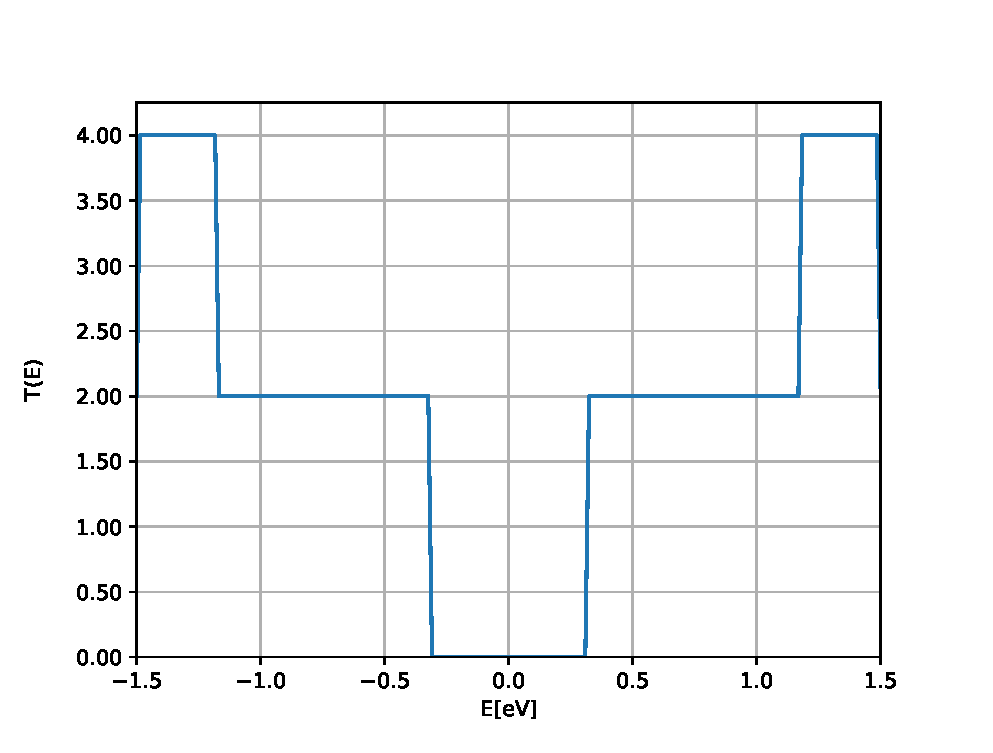
\includegraphics[width=\textwidth]{Figures/NPGNormal_pi.eps}
    \column{.7\textwidth}
    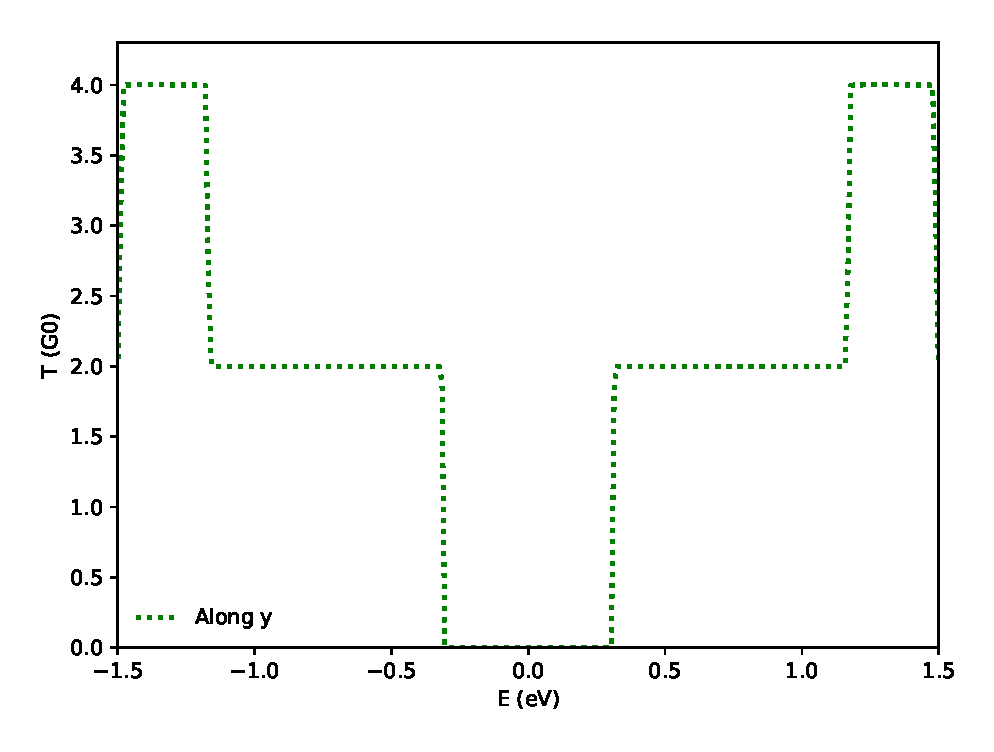
\includegraphics[width=.97\textwidth]{Figures/txy_pi.eps}
\end{columns}
\onslide<3>
\centering
\begin{align*}
		k = \mathrm{AVG}\pqty{0,\frac{\pi}{2},\pi}
\end{align*}
\begin{columns}[t]
    \column{.7\textwidth}
    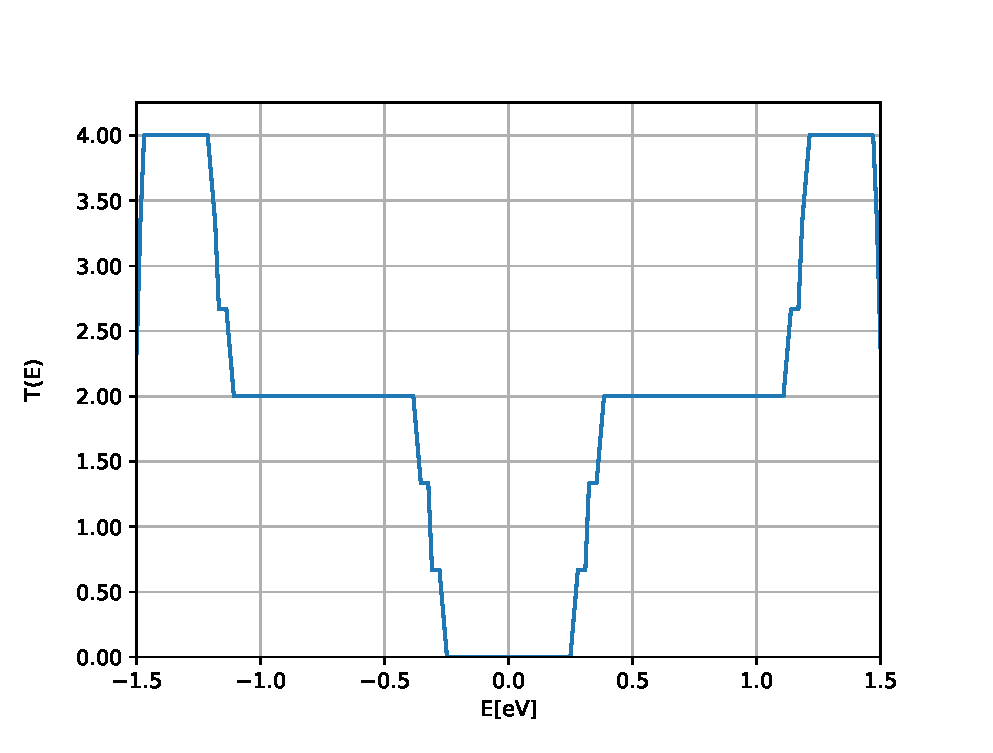
\includegraphics[width=\textwidth]{Figures/NPGNormal_AVER.eps}
    \column{.7\textwidth}
    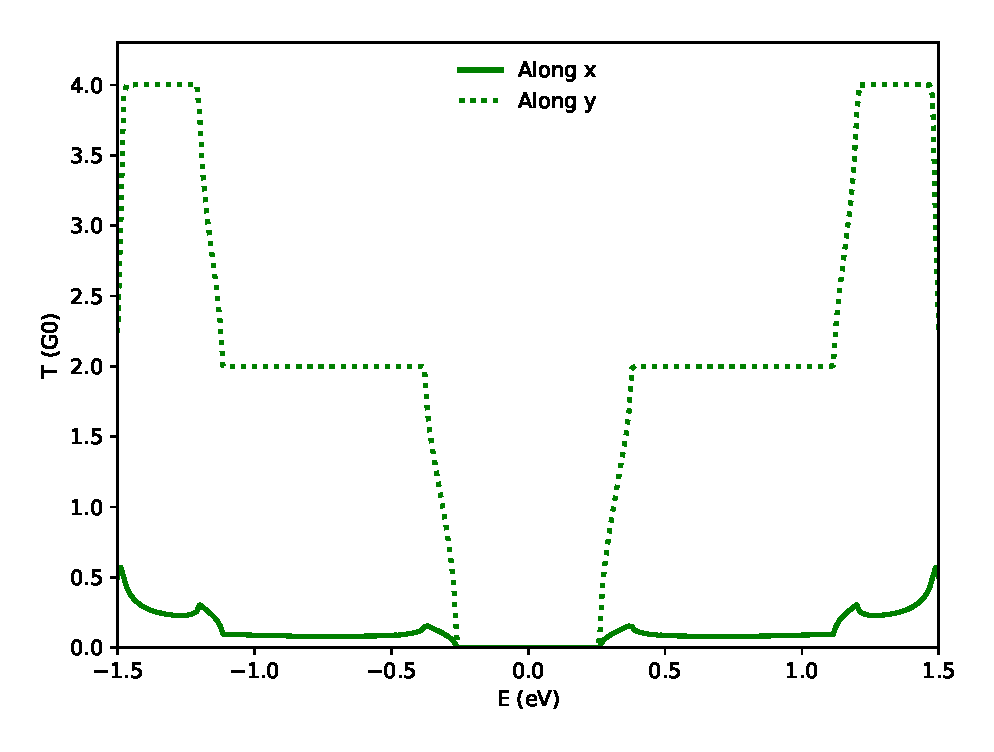
\includegraphics[width=.97\textwidth]{Figures/txy_AVER.eps}
\end{columns}
\end{overprint}
\end{frame}

\begin{frame}{Summary of code structure}
\centering
\includegraphics[width=1.3\textwidth]{Figures/Flowchart.eps}
\end{frame}

\section{Exploring GNR bridges}
\subsection{Para-O\mathinhead{_4}{_4}-NPG, Para-(OH)\mathinhead{_4}{_4}-NPG, Meta-O\mathinhead{_2}{_2}-NPG, Meta-(OH)\mathinhead{_2}{_2}-NPG}

\begin{frame}{Para and meta bridges}
\centering
\begin{overprint}
\onslide<1>
\centering
\begin{columns}[t]
\column{.5\textwidth}
    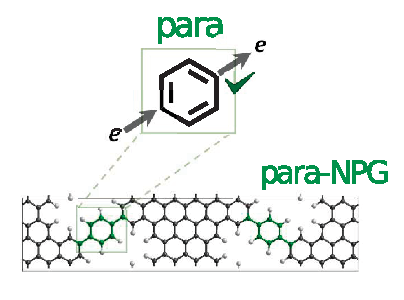
\includegraphics[height=\textwidth]{Figures/Parametagraphic.eps}
\column{.5\textwidth}
    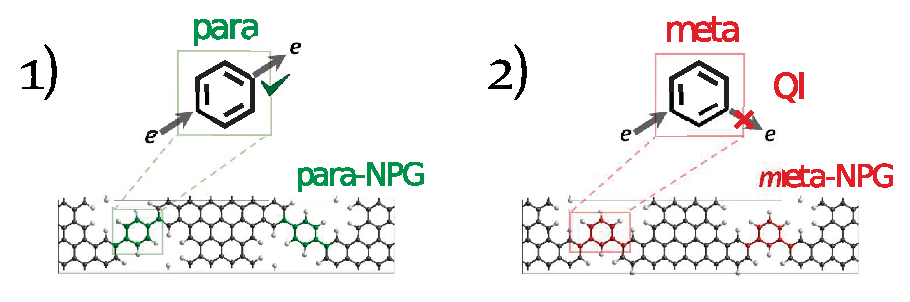
\includegraphics[height=\textwidth]{Figures/Metaparagraphic.eps}
\end{columns}
\onslide<2>
\begin{columns}[c]
    \column{.7\textwidth}
        \begin{itemize}
            \item Path length difference
            \item Quantum interference
            \item Transmission
            \item coupling/decoupling of GNR
        \end{itemize}
    \column{.7\textwidth}
    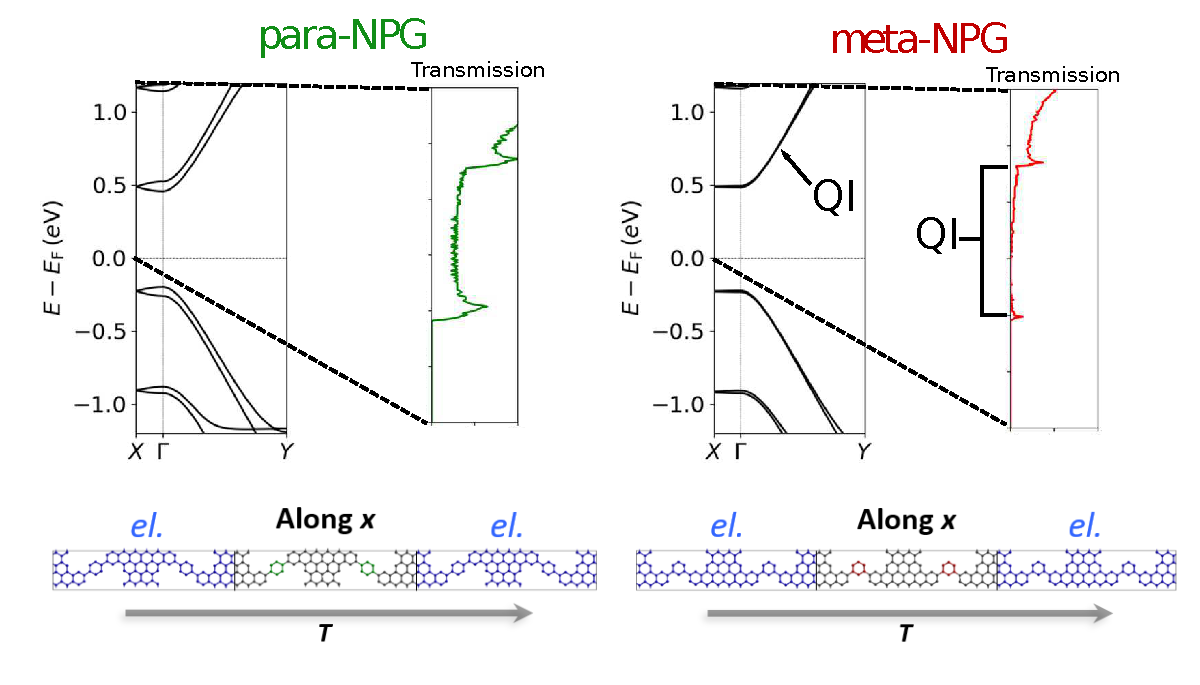
\includegraphics[height=.9\textwidth]{Figures/metapararesultdraft.eps}
\end{columns}
\end{overprint}
\end{frame}

\begin{frame}{Para-O\mathinhead{_4}{_4}-NPG}
\centering
\begin{columns}[c]
    \column{.7\textwidth}
    \begin{itemize}
        \item Functionalisation with oxygen
        \item Quantum inteference at valence band 
        \item Reproducing DFT result
        \item Decoupling of GNR 
        \item Bands at Fermi level
    \end{itemize}
    \column{.7\textwidth}
    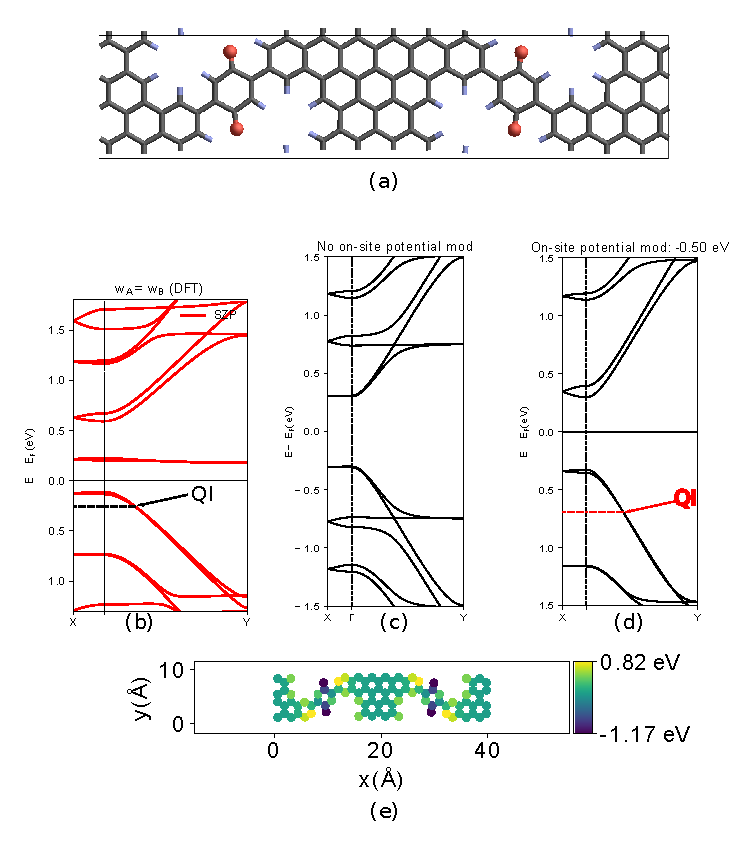
\includegraphics[width=\textwidth]{Figures/fig19.eps}
\end{columns}
\end{frame}

\begin{frame}{Para-(OH)\mathinhead{_4}{_4}-NPG}
\centering
\begin{columns}[c]
    \column{.7\textwidth}
    \begin{itemize}
        \item Hydrogenation of oxygen
        \item Band splitting of DFT
        \item GNR coupling and resemblance with Para-NPG
        \item Reproducing DFT results
    \end{itemize}
    \column{.7\textwidth}
    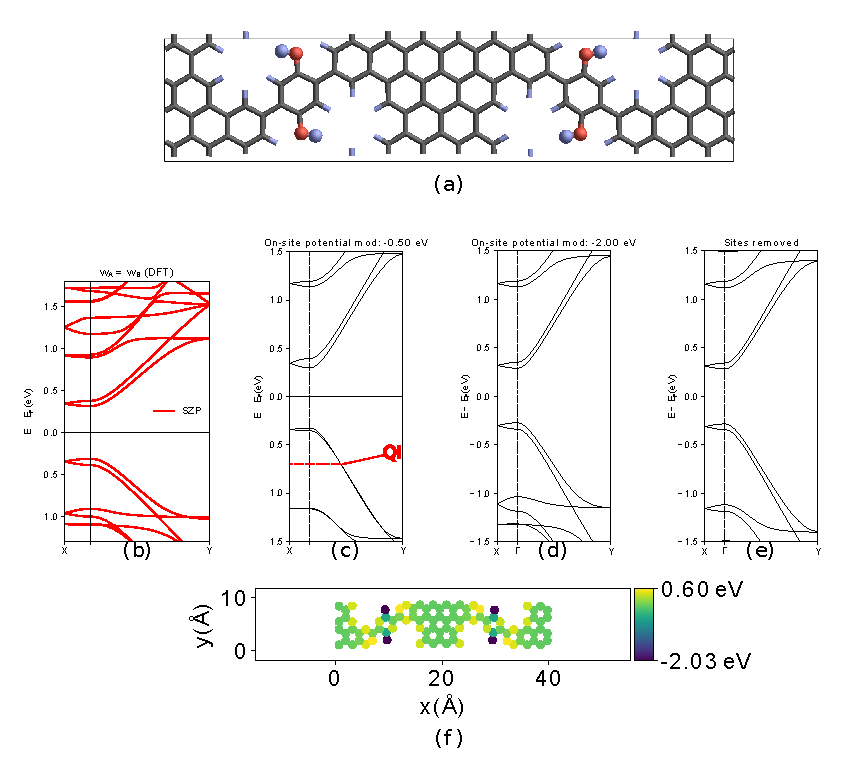
\includegraphics[width=\textwidth]{Figures/fig20.eps}
\end{columns}
\end{frame}

\begin{frame}{Meta-O\mathinhead{_2}{_2}-NPG}
\centering
\begin{columns}[c]
    \column{.7\textwidth}
    \begin{itemize}
        \item Split in the valence for DFT
        \item Similarity in valence/conduction difference for meta/para
        \item Trying different potentials 
        \item Flat bands at Fermi level
    \end{itemize}
    \column{.7\textwidth}
    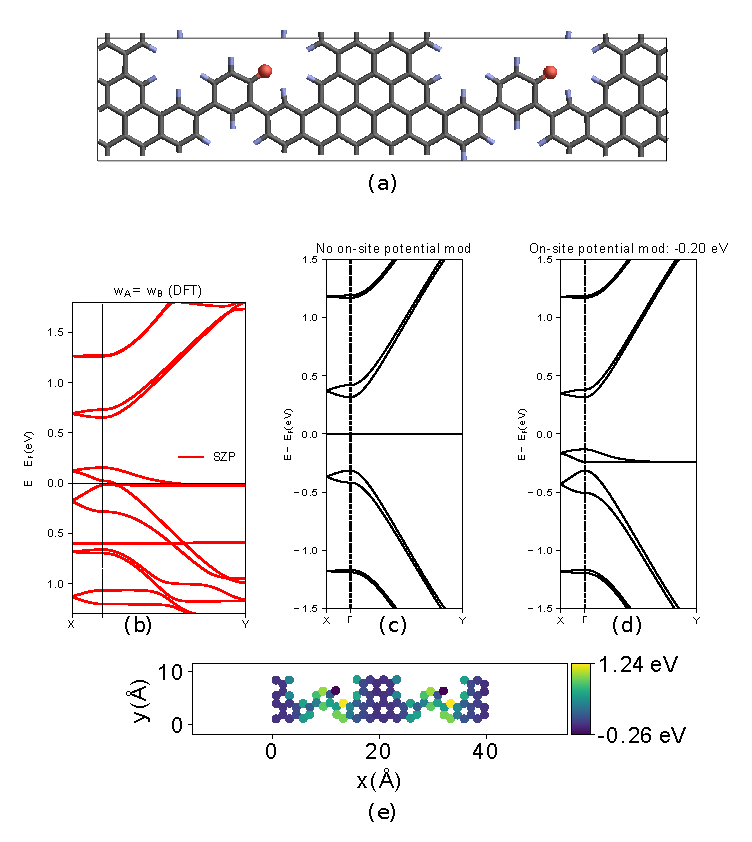
\includegraphics[width=\textwidth]{Figures/fig21.eps}
\end{columns}
\end{frame}

\begin{frame}{Meta-(OH)\mathinhead{_2}{_2}-NPG}
\centering
\begin{columns}[c]
    \column{.7\textwidth}
    \begin{itemize}
        \item 
    \end{itemize}
    \column{.7\textwidth}
    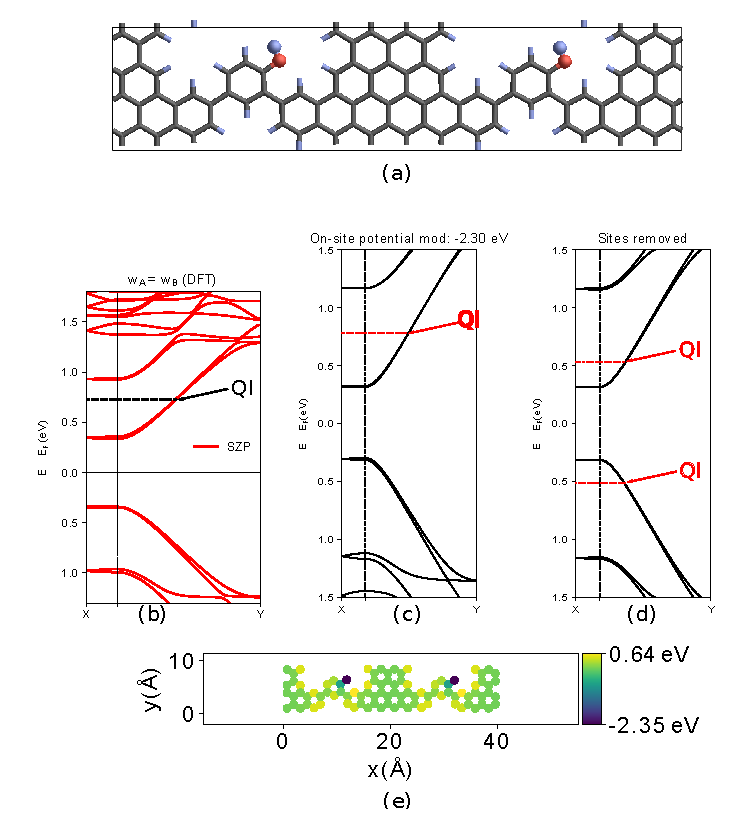
\includegraphics[width=\textwidth]{Figures/fig22.eps}
\end{columns}
\end{frame}

\begin{frame}{Conclusion}
	\centering
	\begin{beamercolorbox}[sep=1em,wd=10cm]{redbox}
		``Development of tight-binding routines in Python in order to understand electron transport in novel nanoporous graphene devices (NPGs)''
	\end{beamercolorbox}
\end{frame}

\section*{Questions}
\title{Questions}
\subtitle{}
\begin{frame}
	\titlepage
\end{frame}

\appendix
\section{Energy and velocity fits}
\begin{frame}{Energy and velocity fits}
	\begin{itemize}
		\item Appendix
	\end{itemize}
\end{frame}

\end{document}
